\documentclass[12pt,oneside,a4paper]{article}
\usepackage{multirow}
\usepackage[table,xcdraw]{xcolor}
\usepackage{outlines}
\usepackage{footnote}
\usepackage{framed}
\usepackage{tablefootnote}
\usepackage{tikz}
\usepackage{url}
\usepackage{pgfplots}
\usepackage{float}
\usepackage[bottom]{footmisc}
\usepackage{float}
\usepackage{parskip}
\usepackage{caption}
\usepackage{subcaption}
\usepackage{caption}
\usepackage{siunitx}
\usepackage{graphicx}
\usepackage{circuitikz,siunitx}
\usepackage{tikz}
\usepackage{gensymb}
\renewcommand{\thefootnote}{\roman{footnote}}

%#################################  PAQUETES UTILIZADOS  ##############################################

\usepackage{t1enc}
%\usepackage[latin1]{inputenc}
\usepackage[spanish]{babel}

\addto\captionsspanish{\renewcommand{\tablename}{Tabla}}

%tikzpicture
\usepackage{tikz}
\usepackage{scalerel}
\usepackage{pict2e}
\usepackage{tkz-euclide}
\usetikzlibrary{calc}
\usetikzlibrary{patterns,arrows.meta}
\usetikzlibrary{shadows}
\usetikzlibrary{external}
\usetikzlibrary{decorations.markings}
\usepackage{pstricks}
\usepackage{multirow, multicol}
\usepackage{makecell}
\usepackage{float}
\usepackage{subcaption}
\usepackage[backend=biber,style=ieee]{biblatex}
\addbibresource{Bibliografia.bib}
\usepackage{csquotes}

%pgfplots
\usepackage{pgfplots}
\pgfplotsset{compat=newest}
%\usepgfplotslibrary{statistics}
%\usepgfplotslibrary{fillbetween}

\usepackage{vmargin}    %Margenes

\usepackage{setspace}   %Interlineado

\usepackage{fancyhdr}   %Encabezados

\usepackage{mathtools, amssymb, amsthm, mathrsfs}

\usepackage{graphicx}

\special{src: 15formdif1.tex}

%################################  OPCIONES DEL DOCUMENTO  ############################################

\theoremstyle{definition}
\newtheorem{teo}{Teorema}[section]
\newtheorem{coro}{Corolario}
\newtheorem{prop}{Proposición}
\newtheorem{defi}{Definición}[section]


\newtheoremstyle{ejjstyle}% Name of the style to be used
  {1em}% Space above
  {1em}% Space below
  {\itshape}% Body font
  {}% Indent amount
  {\bfseries}% Theorem head font
  {.}% Punctuation after theorem head
  {.5em}% Space after theorem head
  {\thmname{#1}\thmnumber{ #2}\thmnote{ #3}}% Theorem head specification (can be customized)

% Apply the custom theorem style to each theorem-like environment
\theoremstyle{ejjstyle}
\newtheorem{ej}{Parte}
\newtheorem{ejj}{Ejercicio}

\newcommand{\espEj}{\vspace*{0.1cm}}        %espaciado entre ejercicios
\newcommand{\espPreEj}{\vspace*{0.3cm}}     %espaciado entre titulo de seccion y ejercicios
\newcommand{\espPostEj}{\vspace*{0.4cm}}    %espaciado entre final de ejercicios y proxima seccion

%  margenes
\setmargins
{2.5cm}                    % margen izquierdo
{1cm}                    % margen superior
{16.5cm}                 % anchura del texto
{23.42cm}                % altura del texto
{15pt}                   % altura de los encabezados
{1cm}                    % espacio entre el texto y los encabezados
{0pt}                    % altura del pie de página
{2cm}                    % espacio entre el texto y el pie de página

%  encabezado y pie de pagina
\pagestyle{fancy}
\fancyhf{}
\rhead{ITBA}
\lhead{Teoría de Circuitos II}
\chead{Caviglia}
\rfoot{\thepage}


\usepackage{hyperref}
\hypersetup{
    colorlinks=true,
    linkcolor=black,
    filecolor=magenta,      
    urlcolor=blue,
    pdfpagemode=FullScreen,
}

%   Settings de pgfplots
\pgfplotsset{
    standard/.style={
    axis line style = thick,
    trig format=rad,
    enlargelimits,
    axis x line=middle,
    axis y line=middle,
    enlarge x limits=0.15,
    enlarge y limits=0.15,
    every axis x label/.style={at={(current axis.right of origin)},anchor=north west},
    every axis y label/.style={at={(current axis.above origin)},anchor=south east}
    }
}


\graphicspath{ {images/} }




\begin{document}

\begin{titlepage}
	\centering
	
\includegraphics[width=0.5\textwidth]{images/Logo Itba.png}\par\vspace{0.5cm}
	{\LARGE Teoría de Circuitos II \par} 
	\vspace{0.5cm}
	{\Large \color{gray} Primer Cuatrimestre de 2024\par}
        \rule{150mm}{0.1mm}
	{\LARGE\bfseries Trabajo Pr\'actico N3\par}
        {\Large\bfseries Grupo 2 \par}
        \subsection*{Conversi\'on de impedancias, instrumentaci\'on, sensado a lazo
        cerrado y ecualizadores}
        \vspace{0.2cm}
        \subsection*{Ejercicio 2: S\'intesis de Carga Activa}
        \rule{150mm}{0.1mm}
        \vspace{0.5cm} \\
	{\LARGE\bfseries\itshape Integrantes}\par \vspace{0.1cm}
        \begin{minipage}[b]{0.4\linewidth}
            \texttt{Facundo Caviglia}\par 
        \end{minipage}
        \begin{minipage}[b]{0.2\linewidth}
            \texttt{63178}\par
        \end{minipage} \\
        \vspace{1cm}
	{\LARGE\bfseries\itshape Profesores}\par \vspace{0.1cm}
        \begin{minipage}[b]{0.4\linewidth}
            \texttt{Petrucci, Javier}\par
            \texttt{Jacoby, Daniel}\par
        \end{minipage}\\
        \vspace{1cm}
	\vfill
	{\large Fecha de entrega: 03/05/2024\par} % heutige Datum
\end{titlepage}


\newpage

\tableofcontents

\newpage

\section{Introducción}
En la electrónica, la manipulación de una impedancia es fundamental para adaptar señales 
entre distintos componentes o circuitos. Uno de los dispositivos más utilizados en este ámbito 
para lograr esta adaptación es el potenciómetro: una pieza versátil que permite hacer variar el valor 
de una resistencia de manera controlada mediante un eje giratorio. 

En este trabajo práctico se hará uso del transistor \textbf{MOSFET} y el amplificador 
operacional \textbf{TL082} (opamp). Con estos componentes se puede diseñar un circuito capaz de modificar su impedancia 
de entrada de manera dinámica y manual. Este trabajo práctico se enfocará en combinar estos componentes 
en un circuito para lograr un circuito con impedancia de entrada variable, controlada mediante un potenciómetro.

\subsection*{Objetivo}
Como se mencionó anteriormente, el objetivo de este trabajo práctico es diseñar un circuito 
que permita modificar su impedancia de entrada de manera controlada. Además, se quiere lograr 
una resistencia variable que pueda soportar una cantidad de corriente considerable, en el orden de los 
Amperes. Si bien existen potenciómetros con resistencia variable que resisten una corriente significante como 
1A, estos tienen un tamaño muy grande en comparación a los potenciómetros comunes.

De esta manera, se propone diseñar un circuito que permita modificar la resistencia de entrada 
y además soportar una corriente considerable. También, se busca que el circuito tenga un tamaño
reducido y sea fácil de implementar.

En este trabajo práctico se explorará el comportamiento del circuito propuesto y se analizará
su respuesta en frecuencia. Se llevará a cabo un desarrollo teórico utilizando sistemas 
realimentados y se realizarán algunas aproximaciones que serán explicadas en detalle en la 
sección de desarrollo teórico.

\section{Materiales Utilizados}
Para llevar a cabo este experimento se hará uso de un transistor MOSFET, un opamp TL082, y un potenciómetro
de 100k$\Omega$.

¿Qué es un MOSFET? En principio cabe destacar el funcionamiento y aplicación de un transistor MOSFET.
El Metal Oxide Semiconductor Field-Effect Transistor es un dispositivo 
semiconductor que controla el flujo de corriente entre dos terminales, denominados Drain (Drenaje) 
y Source (Fuente), mediante la aplicación de un voltaje en una tercera terminal llamada Gate (Compuerta).

Su funcionamiento se basa en el control del campo eléctrico en una región del semiconductor, denominada 
canal, que conecta las terminales de fuente y drenaje. La aplicación de un voltaje en la compuerta
modifica la conductividad del canal, permitiendo o bloqueando el flujo de corriente entre las terminales
de fuente y drenaje. De esta manera, el MOSFET permite controlar la corriente que circula entre sus terminales 
de manera controlada.

A continuación se presenta el diagrama de un MOSFET de canal N, que es el tipo de transistor que se utilizará 
en este trabajo práctico. Se presentan las terminales para mejor comprensión.

\begin{figure}[H]
    \centering
    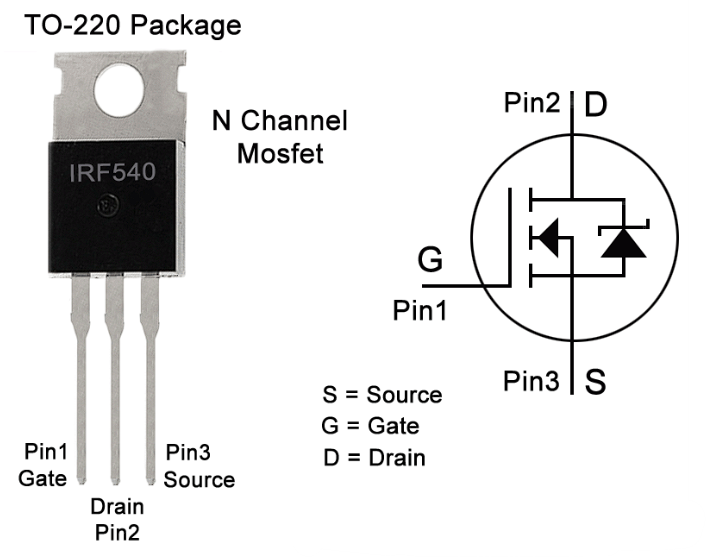
\includegraphics[width=0.5\textwidth]{images/MOSFET.png}
    \caption{Diagrama de un MOSFET de canal N}
\end{figure}

Se estima que la corriente que circula en la terminal de drenaje es igual a la corriente que circula
en la terminal de fuente dado a que la corriente que circuila por el terminal de compuerta es casi 0. 
La siguiente ecuación describe el comportamiento del MOSFET:

\begin{equation}
    I_S \approx I_D = K \cdot (V_{GS} - V_{TH})^2
\end{equation}

Donde $ K = \frac{gm}{2\cdot (V_{GS} - V_{TH})} $, $ gm $ es la transconductancia del MOSFET, $ V_{GS} $ 
es la tensión entre la compuerta y la fuente, y $ V_{TH} $ es la tensión umbral del MOSFET dada por 
el fabricante en su hoja de datos. En este experimento, 
se hará uso de un transistor \textbf{IRF540}. Según su hoja de datos, la transconductancia típica del transistor 
es de 8,7$\frac{1}{\Omega}$ y la tensión de umbral es de 2,9V.

Por lo tanto queda:

\begin{equation}
    I_S \approx I_D = \frac{gm}{2\cdot (V_{GS} - V_{TH})} \cdot (V_{GS} - V_{TH})^2 = \frac{gm}{2} \cdot (V_{GS} - V_{TH})
\end{equation}

Como se había mencionado, se utilizará el opamp TL082. Este dispositivo es un amplificador operacional 
de alta impedancia de entrada y baja impedancia de salida. Su funcionamiento se basa en la amplificación 
de la diferencia de tensión entre sus terminales de entrada. 

En los anteriores trabajos prácticos se investigó y estudió el comportamiento, cualidades, 
aplicaciones y limitaciones del mismo. En este trabajo práctico se hará uso de este dispositivo 
para controlar la tensión de gate del MOSFET. Además, recordar que si el opamp mantiene una 
realimentación negativa, se obtiene una masa virtual la cual es beneficiosa para este experimento.

\newpage 

El componente más importante de este experimento es el potenciómetro. Se utilizará una resistencia variable 
de 100k$\Omega$ con el fin de modificar la impedancia de entrada del circuito. 
Un potenciómetro tiene tres terminales: dos extremos y un terminal central. Los dos extremos están
conectados a una resistencia fija, mientras que el terminal central se conecta a un eje rotatorio. 
De esta manera, se puede modificar la resistencia total del potenciómetro variando la posición del eje. 
También, este método permite ajustar un divisor resistivo de manera controlada. 

En este trabajo práctico se utilizará el eje rotatorio del potenciómetro para modificar la 
resistencia de entrada del circuito. Se denomina como $k$ a la posición del cursor, donde $0 \leq k \leq 1$.
En la siguiente sección se presentará el circuito propuesto y se explicará su funcionamiento. Se 
explicará como la variable $k$ se relaciona con la resistencia de entrada del circuito.

Por último, se deben mencionar los componentes o fuentes restantes que se utilizarán para que el 
experimento pueda llevarse a cabo. Se utilizará una fuente de alimentación de $\pm 15V$ para el opamp, un 
osciloscopio para medir las señales de entrada y salida, y una fuente de tensión continua $V_D$ para
polarizar el MOSFET y establecer el \enquote*{Q-point} del mismo.
Este valor de tensión se determinará en la sección de desarrollo teórico, ya que dependiendo de la corriente 
que se quiera obtener, deberá ajustarse la entrada. Es importante tener en cuenta 
que la fuente de tensión que se encuentra en el laboratorio no soporta una corriente mayor a 3A. 

Luego, es importante destacar que la tensión que se aplique en la compuerta del MOSFET 
hace variar la corriente que circula por el drenaje y la fuente. Sin embargo, hay que recordar que 
la tensión máxima que soporta la salida del opamp es de $\pm 13V$, por lo que hay que tener cuidado 
a la hora de analizar el circuito, ya que es posible que el opamp se encuentre saturado.

\section{Desarrollo Teórico}
Con el fin de comprender el funcionamiento del circuito propuesto, se realizará un análisis del sistema 
en cuestión. Primero, se recuerda que el parámetro que se quiere controlar es la impedancia de entrada 
del circuito. 

Para calcular el mismo, se hará uso de la siguiente ecuación: 

\begin{equation}
    Z_{in} = \frac{V_{in}}{I_{in}} = \frac{V_D}{I_{D}}
\end{equation}

De esta manera, puede calcularse la impedancia de entrada del circuito en función de la corriente que circula 
por el drenaje del MOSFET. Ya sabiendo la tensión de entrada, hace falta encontrar una ecuación que determine 
la corriente $I_D$. Se verá luego en las ecuaciones que esta corriente dependerá de la posición del cursor 
del potenciómetro. Esta variable se denomina como $k$, y se propone encontrar una función transferencia que 
relacione la impedancia de entrada con la posición del cursor. 

\newpage

Se quiere encontrar la siguiente función transferencia:

\begin{equation}
    H(s) = \frac{Z_{in}(s)}{k(s)}
\end{equation}

Sin embargo, por fines prácticos del desarrollo teórico, se encontrará la admitancia de entrada en función 
del cursor $k$. Esto facilita el desarrollo de la función transferencia a través de un 
un análisis de sistemas realimentados.

Se recuerda que la admitancia es:

\begin{equation}
    Y_{in} = \frac{1}{Z_{in}} = \frac{I_{in}}{V_{in}} = \frac{I_{D}}{V_{D}}
\end{equation}

Por lo que la función transferencia a encontrar es:

\begin{equation}
    H(s) = \frac{Y_{in}(s)}{k(s)}
\end{equation} 

\subsection*{Circuito a estudiar}

Habiendo declarado los objetivos del trabajo práctico, mencionado los componentes esenciales, y 
explicados los parámetros importantes del circuito con sus respectivas ecuaciones, se procede a 
presentar el circuito propuesto:

\begin{figure}[H]
    \centering
    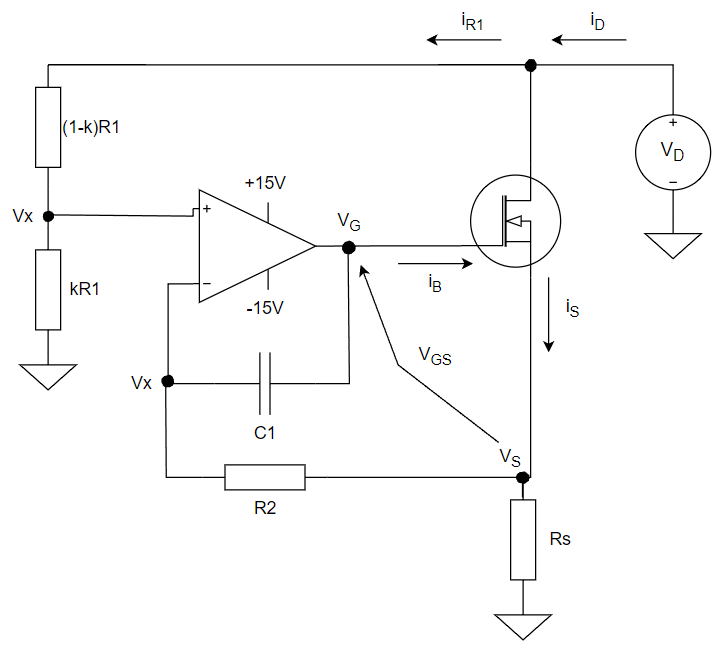
\includegraphics[width=0.7\textwidth]{images/CircuitoTC.png}
    \caption{Circuito propuesto}
\end{figure}

\subsection*{Criterio de Elección de Componentes}

En la siguiente tabla pueden verse los valores de los componentes utilizados en el circuito:

\begin{table}[H]
    \centering
    \begin{tabular}{|c|c|}
    \hline
    \rowcolor[HTML]{C0C0C0} 
    \textbf{Componente} & \textbf{Valor} \\ \hline
    $R_1$               & 100k$\Omega$     \\ \hline
    $R_2$               & 10k$\Omega$     \\ \hline
    $R_S$               & 1$\Omega$     \\ \hline
    $C_1$               & 10nF     \\ \hline
    \end{tabular}
\end{table}

Se recuerda que el potenciómetro utilizado es de 100k$\Omega$, y no puede manejar corrientes en el orden 
de los amperes. Por lo tanto, se eligió una resistencia muy elevada en comparación a la resistencia de 
carga para que la corriente que circule por el potenciómetro sea despreciable. De esta manera, se puede 
considerar que:

\begin{equation}
    I_{R_1} + I_D \approx I_D
\end{equation}

Además, el MOSFET tiene la cualidad de que por la terminal de compuerta circula una corriente
en el orden de los nA, por lo que se considera que no circula corriente. Así, se puede 
asumir que la corriente que circula por el drenaje es igual a la corriente que circula por la fuente.

Como se había mencionado anteriormente:

\begin{equation}
    I_B + I_D = I_S \implies I_S \approx I_D = \frac{gm}{2} \cdot (V_{GS} - V_{TH})
\end{equation}

La resistencia de carga o de fuente es $R_S = 1\Omega$, lo que quiere decir que es una resistencia 
de potencia capaz de soportar corrientes en el orden de los amperes. Se eligió una resistencia de 
alambre bobinado de 10W para que pueda soportar una corriente máxima de 3A. La ecuación de potencia 
establece que:

\begin{equation}
    P = I^2 \cdot R \implies 3^2 \cdot 1 = 9W
\end{equation}

Con el fin de establecer un valor de la fuente de tensión continua $V_D$, se debe hacer un análisis de 
previo con el comportamiento del MOSFET. Se sabe que la tensión umbral del transistor es de 2,9V,
por lo que se debe establecer un potencial $V_{GS}$ mayor a este valor. Además, 
como se quiere obtener una corriente de 3A, se debe ajustar la tensión de entrada de manera que 
la corriente que circule por el drenaje sea de 3A.

\begin{equation}
    V_S = I_S \cdot R_S = 3 \cdot 1 = 3V
\end{equation}

Se recuerda que el MOSFET empieza a conducir cuando la tensión entre la compuerta y la fuente $V_{GS}$ supera el 
voltaje umbral $V_{TH}$. Es decir, el MOSFET comenzará a permitir el paso de corriente del drenaje a la fuente 
cuando $V_{GS} > V_{TH}$. 

Por lo tanto:

\begin{equation}
    V_G - V_S > V_{TH} \iff V_G > V_S + V_{TH} \iff V_G > 5,9V
\end{equation}

De esta manera, se tiene que establecer como mínimo una tensión de 5,9V en la compuerta del MOSFET para que 
este pueda conducir y lograr una corriente máxima de 3A en la resistencia de carga. Mediante simulaciones 
de LTSpice se hicieron pruebas para establecer un valor en la fuente de tensión continua $V_D$ que permita
obtener una corriente de 3A. Teniendo en cuenta el caso en que k = 1, el potenciómetro no genera 
un divisor resistivo entre la terminal no inversora del opamp y la entrada. Esto quiere decir que, 
debido a la masa virtual del opamp, habrá la misma caída de potencial entre la resistencia de 
carga que la tensión de entrada. 

Por lo tanto, se concluyó que la tensión de entrada debe ser de 3V para obtener una corriente máxima de 3A. 
Haciendo variar k se puede obtener una corriente menor que circule por la resistencia de carga. Además, se
pudo ver en las simulaciones que la tensión $V_{GS}$ siempre se mantuvo por encima de 5,9V, que era 
el resultado que se deseaba.

La resistencia será capaz de soportar esta corriente, disipando una potencia de 9W y generando calor 
en la misma. Se recomienda siempre tomar en cuenta la temperatura de todos los componentes, y no 
pasarse de los límites eléctricos de los mismos. Todos los componentes suelen tener una hoja de datos 
donde se especifican los límites eléctricos y térmicos de los mismos. Si se excede de estos límites se pueden 
generar daños en los componentes y en el circuito en general. 

En este caso la resistencia está preparada para soportar esta magnitud de corriente sin sobrecalentarse. 
Sin embargo, es muy importante tener en cuenta que los transistores son componentes que se calientan 
significativamente cuando conducen corrientes altas. El IRF540 viene en un encapsulado TO-220 que no le 
permite disipar el calor por su cuenta de manera eficiente. Es por esto que el encapsulado viene con un 
espacio para colocar un disipador de calor. En este experimento se utilizará un disipador de extrusión 
de aluminio para disipar el calor generado por el transistor. En la siguiente sección se especificarán 
los límites térmicos del transistor.

\newpage
\subsection*{Oscilaciones} 
Es importante tener en cuenta que el circuito propuesto es conocido por generar 
oscilaciones en la salida. Esto puede ser causado por el ruido ambiental de 50 Hz que es captado por el 
osciloscopio, o que el MOSFET es un dispositivo que puede oscilar si no se
controla correctamente. En este caso, se utilizará un opamp para controlar la tensión de gate del MOSFET, 
y además se colocará un circuito integrador para evitar oscilaciones en la salida. Se recomienda para este 
experimento utilizar un capacitor y una resistencia como se puede ver en la \enquote*{Figura 2} para 
evitar oscilaciones en la salida.

Como estos componentes fueron utilizados solamente con el propósito de evitar oscilaciones, el 
desarrollo teórico para conseguir la función de transferencia requerida no se verá afectado por la 
presencia de estos componentes. Tendremos en cuenta que ambos componentes estarán fuera del circuito:
el capacitor desconectado, es decir, abierto, y la resistencia en corto.

Luego de haber implementado el circuito y llevado a cabo el experimento práctico,
se observó que en el osciloscopio igualmente había ruido en la salida. Por lo tanto se decidió 
quitar esta resistencia, dejando solamente el capacitor. Al hacer este cambio, se pudo observar que
las oscilaciones disminuyeron considerablemente, casi desapareciendo. Por lo tanto, es importante 
destacar que de ahora en adelante se tendrá en consideración que el circuito no posee la resistencia 
$R_2$

\subsection{Función Transferencia}

Para encontrar la función transferencia $H(s)$, se debe encontrar la admitancia de entrada
en función de la posición del cursor $k$. Es importante recordar que la resistencia y capacitor 
que fueron colocadas para evitar las oscilaciones no serán tenidas en cuenta en este desarrollo teórico.
Luego de analizar la función transferencia teórica, para estudiarla de manera práctica se 
llevará a cabo el mismo experimento pero posicionando una resistencia en paralelo a la $kR_1$. De 
esta manera, se generará un divisor resistivo dependiendo también de esta nueva resistencia.

Por esta razón es que se decide estudiar el comportamiento de la admitancia de entrada en función de 
una constante $k$, que si se coloca esta resistencia extra, esta constante ya no será equivalente 
a la posición del curso, sino que al factor que multiplica el divisor resistivo.

Con el fin de analizar el circuito, se propone primero encontrar la relación de este divisor resistivo.
Ver la \enquote*{Figura 2} para mejor comprensión.

\begin{equation}
    V_{X} = V_D \cdot \frac{k R_1}{k R_1 + (1-k)R_1} = V_D \cdot k
\end{equation}

Notar que esta ecuación es válida para la figura en cuestión. Luego si se agrega la resistencia en 
paralelo tendrá que usarse esta misma ecuación, y se tomará $k$ como la misma constante que antes. 
Si se da una situación donde se pudiera activar instantáneamente la resistencia en paralelo,
se efectuaría un salto en la constante k, por lo que puede ser tomado como un escalón. Es así como 
en la siguiente sección se podrá comparar la función transferencia teórica con la práctica.

A continuación se muestra el circuito que será estudiado de manera teórica:

\begin{figure}[H]
    \centering
    \includegraphics[width=0.75\textwidth]{images/Circuito2.png}
    \caption{Circuito propuesto}
\end{figure}

\subsection*{Sistemas Realimentados}
Para el análisis de la admitancia de entrada en función de $k$, se propone el siguiente análisis de 
sistemas realimentados. Recordar que el parámetro a variar es esta constante, por lo que será lo 
primero que se tomará en cuenta. Se puede llegar al siguiente sistema:

\begin{figure}[H]
    \centering
    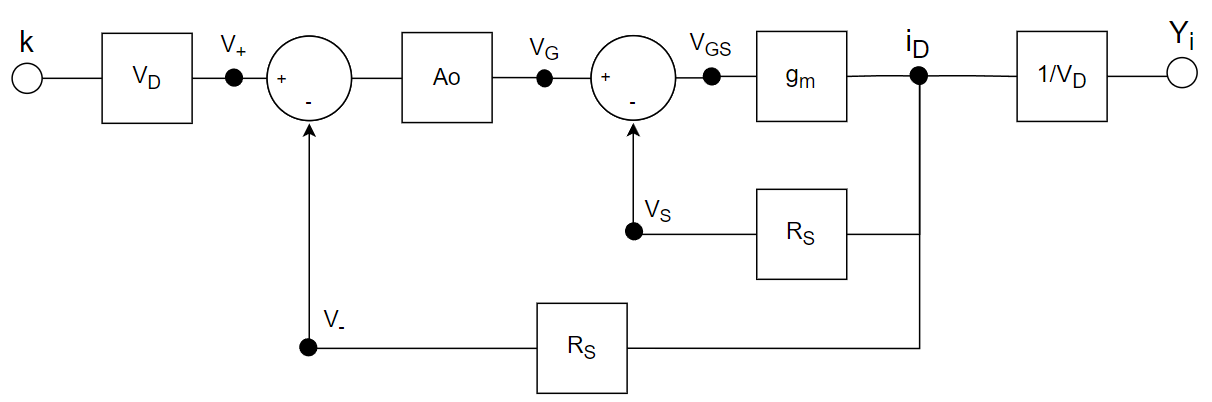
\includegraphics[width=1\textwidth]{images/realim1.png}
    \caption{Sistema realimentado completo}
\end{figure}

\newpage
Haciendo variar la constante k, se puede cambiar el divisor resistivo entre la entrada y $V_+$. Luego, el 
operacional se encarga de establecer una tensión de salida $V_G$ mediante la realimentación negativa. 
Como ya sabemos, esta ecuación es dada por:

\begin{equation}
    V_G = A_o(V_+ - V_{-})
\end{equation}

Se debe tomar en cuenta el hecho de que el operacional no es ideal y tiene una ganancia $A_v$ finita que 
varía con la frecuencia. Sin embargo, para este análisis se tomará como ideal.

Luego de la operación dada por el opamp, viene el efecto causado por el MOSFET. Según la tensión
que se aplica en la compuerta, deja pasar una cierta cantidad de corriente $I_D$ hacia la resistencia 
de carga. Como puede verse en la figura, la tensión entre la compuerta y fuente no es estrictamente $V_G$, sino 
que es $V_G - V_S$. Esto quiere decir que debe llevarse a cabo otra realimentación negativa para 
poder llegar a la relación entre k y la corriente $I_D$. 

Una vez llegado a este punto, se puede encontrar la relación entre la corriente $I_D$ y la constante $k$.
Así, lo único que queda es dividir esta corriente por la tensión de entrada $V_D$ para encontrar la 
admitancia de entrada en función de $k$. De esta manera se completa el análisis de la función transferencia 
deseada por sistemas realimentados.

Con el fin de obtener la relación entre la admitancia y la constante k, se debe analizar cada 
parte del sistema por separado. Primero se deben analizar los casos realimentados negativamente 
y luego se puede armar un sistema más simple. A continuación se muestra un sistema de realimentación 
negativa simple para poder calcular su transferencia:

\begin{figure}[H]
    \centering
    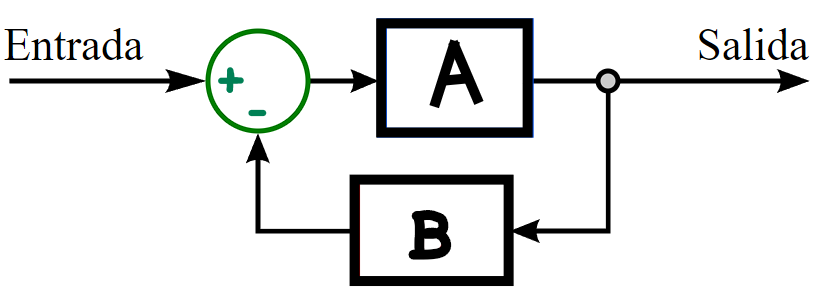
\includegraphics[width=0.6\textwidth]{images/realim3.png}
    \caption{Sistema realimentado simple}
\end{figure}

Puede llegarse a la siguiente expresión:

\begin{equation}
    H(s) = \frac{1}{B} \cdot \frac{AB}{1 + AB}
\end{equation}

De esta manera, también se puede llegar a la siguiente aproximación:

\begin{equation}
    H(s) = \frac{1}{B} \cdot \frac{AB}{1 + AB} \approx \frac{1}{B} \iff A \rightarrow \infty
\end{equation}

Por lo tanto, se puede llegar a despreciar el factor que multiplica a $\frac{1}{B}$ si el término 
$\frac{AB}{1 + AB}$ tiende a 1.

Como se pudo analizar el caso de una realimentación negativa simple, a continuación se provee 
un sistema menos complejo derivado del anterior:

\begin{figure}[H]
    \centering
    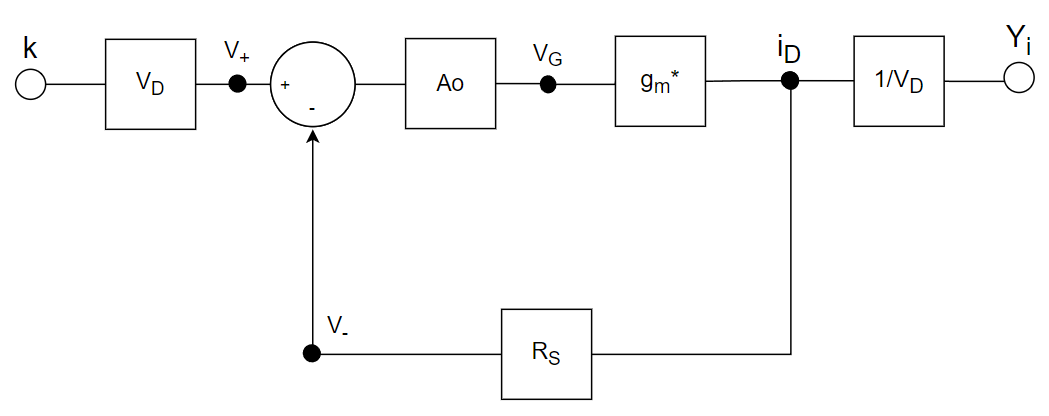
\includegraphics[width=1\textwidth]{images/realim2.png}
    \caption{Sistema realimentado}
\end{figure}

Donde se toma la siguiente simplificación:
\begin{equation}
    g_m^* = \frac{1}{R_S} \cdot \frac{g_m R_S}{1 + g_m R_S}
\end{equation}

Se mostrarán a continuación la serie de ecuaciones necesarias para llegar a la función transferencia
final.

\begin{equation}
    H(s) = \frac{Salida}{Entrada} = \frac{Y_i(s)}{k(s)}
\end{equation}

\begin{equation}
    k\cdot V_D \cdot H_1(s) \cdot \frac{1}{V_D} = Y_i(s) \iff \frac{Y_i(s)}{k(s)} = H_1(s)
\end{equation}

\begin{equation}
    H(s) = H_1(s) = \frac{1}{R_S}\cdot \frac{A_o\cdot g_m^*\cdot R_S}{1 + A_o\cdot g_m^*\cdot R_S}
\end{equation}

De esta manera, para despejar la impedancia de entrada $Z_i$ que estabamos buscando:

\begin{equation}
    Y_i = \frac{k}{R_S} \cdot \frac{A_o\cdot g_m^*\cdot R_S}{1 + A_o\cdot g_m^*\cdot R_S} \approx \frac{k}{R_S}
\end{equation}

\begin{equation}
    Z_i = \frac{1}{Y_i} = \frac{R_S}{k}
\end{equation}

Finalmente, se llega a lo que se estaba buscando. Puede verse que el circuito emplea todo un sistema para 
que la impedancia de entrada sea controlada por una constante $k$. En el caso de que no se cambie nada en el 
circuito, esta impedancia de entrada puede ser modificada simplemente con el eje rotatorio del potenciómetro. 
Es una impedancia variable que puede ser controlada de manera manual, y que puede soportar hasta un máximo de 
3 amperes cuando antes no podría. 

Como conclusión, se puede decir que el circuito propuesto es un circuito que permite modificar su impedancia 
de entrada de manera controlada. Sin embargo, es importante destacar la utilidad y practicidad que puede 
llegar a tener este circuito. Si se desea cambiar la impedancia de entrada para que tenga un valor específico, 
es complicado haciéndolo de manera manual por el hecho de que la impedancia cambia muy poco hasta que se llega 
a un cierto valor. Si se analiza la función en relación a la posición del cursor, se puede ver que la función 
cambia muy poco hasta acercarse mucho a 1. Esto quiere decir que fácilmente se podría cambiar la impedancia 
de entrada hasta 4$R_S$, pero por arriba de este valor es muy complicado de controlar.

Cabe aclarar que este análisis se realizó teniendo en cuenta que la corriente que pasa por el potenciómetro 
es despreciable. Si se quisiera llevar a cabo un análisis más preciso, se debería tener en cuenta esta 
corriente, ya que de esta manera $I_D$ no sería igual a 0 cuando $k = 0$, sino que $I_D = I_{R1} =\frac{V_D}{100k\Omega}$.
Por lo tanto, se puede concluir que la impedancia de entrada máxima que se puede obtener es de 100k$\Omega$, 
es decir, del valor del potenciómetro. Esto mismo quiere decir que si se colocase un potenciómetro de 
mayor valor, se podría obtener una impedancia de entrada mayor.

A continuación se presenta la función graficada para poder ver de manera clara el comportamiento de la
impedancia de entrada en función de la posición del cursor.

\begin{figure}[H]
    \centering
    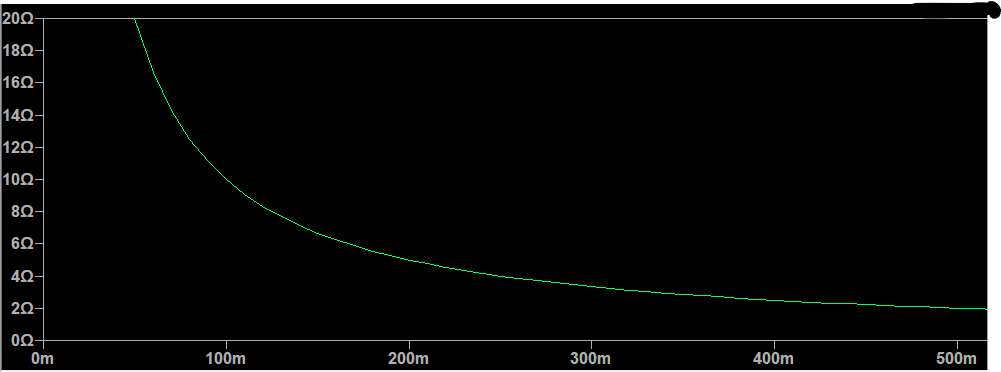
\includegraphics[width=0.8\textwidth]{images/graf.png}
    \caption{Impedancia de entrada en función de la posición del cursor}
\end{figure}

Recordar que k puede tomar valores entre 0 y 1, por lo que el valor final de esta impedancia es 1. 
Además, a medida que k se acerca a 0, esta impedancia se va al infinito (idealmente). Lo que quiere decir 
que si se coloca el cursor en la posición 0, estaría abriendo el circuito y no permitiría el paso de corriente.

\newpage
\subsection*{Aproximaciones Realizadas}

Por último, se desea aclarar que se hicieron algunas aproximaciones ideales para poder llegar a la función 
requerida. Se despreciaron algunos términos que no afectaban significativamente el resultado final, y 
además se asumió que el opamp era ideal. Sin embargo, en la práctica, el opamp no es ideal y tiene una 
ganancia finita que varía con la frecuencia. Pero, al trabajar en una tensión de entrada continua, esto 
quiere decir que la frecuencia es 0, por lo que sí está permitido el uso de la ganancia $A_o$ 
También, se tomó en cuenta la siguiente aproximación en la realimentación negativa:

\begin{equation}
    \frac{A_o\cdot g_m^*\cdot R_S}{1 + A_o\cdot g_m^*\cdot R_S} \approx 1
\end{equation}

Pero, ¿es esta expresión verdadera? Para poder responder a esta pregunta, se realizará su debido 
análisis. Se sabe que la ganancia de un opamp es $A_o = 10^5$ y la transconductancia del MOSFET 
se puede encontrar en la hoja de datos del mismo, pero también se puede calcular mediante la siguiente
fórmula:

\begin{equation}
    g_m = \frac{\Delta I_D}{\Delta V_{GS}} = \frac{2\cdot I_D}{V_{GS} - V_{TH}} = 8,7\frac{1}{\Omega}
\end{equation}

Sin embargo, como se desconocen los métodos de prueba que el fabricante utiliza para medir la 
transconductancia, se llevarán a cabo algunas simulaciones para poder encontrar el valor de la 
misma mediante el uso de LTSpice. Según la hoja de datos, se espera que la tensión $V_{GS}$ sea 
como mínimo de 4,5V para que el transistor pueda conducir. Además, hay que tener en cuenta que 
la tensión $V_G$ no puede ser mayor a 13V, ya que saturaría el opamp. Por lo tanto, para llegar a una zona 
de saturación del MOSFET que permita utilizar la expresión mencionada anteriormente, se eligieron 
los valores de:

\begin{equation}
    g_m = \frac{5A - 3,5A}{5,44V - 5,2V} = 6,25 \frac{1}{\Omega}
\end{equation}

Por lo tanto, se puede calcular el valor de $g_m^*$:

\begin{equation}
    g_m^* = \frac{1}{R_S} \cdot \frac{g_m R_S}{1 + g_m R_S} = \frac{1}{1} \cdot \frac{6,25}{1 + 6,25} = 0,862
\end{equation}

De esta manera, queda:

\begin{equation}
    \frac{A_o\cdot g_m^*\cdot R_S}{1 + A_o\cdot g_m^*\cdot R_S} = \frac{10^5 \cdot 0,862 \cdot 1}
    {1 + 10^5 \cdot 0,862 \cdot 1} = 0,99999
\end{equation}

Se puede concluir que en definitiva este término es aproximadamente 1, por lo que la aproximación
realizada es válida. Por lo tanto, se puede afirmar que la función transferencia encontrada es
válida para el circuito propuesto.

\subsection{Limitaciones Eléctricas}
En esta sección se presentarán las limitaciones eléctricas de los componentes utilizados en el circuito.
Como se había mencionado anteriormente, es esencial mantener a los componentes pasivos y activos dentro de 
sus límites eléctricos para evitar daños en los mismos. Existe un rango de utilidad para todos los componentes 
que se utilizan en cada circuito. Por ejemplo, las resistencias tienen un rango de tolerancia que hace variar 
su valor nominal en función de la temperatura. También, existen resistencias de metal film o carbon film que 
son fabricadas de una cierta manera, para ciertas potencias. Por ejemplo, si se utilizara una resistencia de 
1/4W en lugar de una de 10W para este experimento, esta se quemaría, causando posibles daños en el circuito.

El otro componente que debe manejar altas corrientes y por lo tanto temperaturas, es el transistor MOSFET. 
Este componente es un semiconductor que puede llegar a calentarse mucho si se le aplica una corriente 
considerable. En la hoja de datos de los transistores se puede observar las características térmicas del 
componente y la temperatura máxima que puede soportar. En este caso, el transistor IRF540 suele operar 
a una temperatura de 175°C, por lo que se debe tener en cuenta que si se excede esta temperatura.

Para hacer un análisis del manejo térmico en circuitos eléctricos, primero hace falta comprender algunas 
de las ecuaciones que las rigen:

\begin{equation}
    Q \cdot R_{\theta} = \Delta T
\end{equation}

Donde $Q$ es la potencia disipada por el componente, $R_{\theta}$ es la resistencia térmica total del componente,
y $\Delta T$ es la variación de temperatura en el componente. La resistencia térmica es una característica
de los componentes que indica cuánto se calienta el componente por cada watt que disipa. Sin colocar un 
disipador, este tipo de componentes mantienen una resistencia conocida como $R_{\theta JA}$, que es la
resistencia térmica entre el componente y el ambiente. 

Si se observa en la hoja de datos, el IRF540 tiene 
una resistencia térmica juntura-ambiente de 62°C/W. Si se coloca un disipador de calor, esta resistencia
térmica disminuye considerablemente. Existen 3 resistencias térmicas distintas: juntura-carcaza, 
carcaza-disipador, y disipador-ambiente. En total, esta resistencia equivalente (serie) tiene un valor 
mucho menor que el de la resistencia térmica juntura-ambiente. Por lo tanto, deja pasar más calor y 
puede disipar más potencia. 

En este experimento, se quiere hacer pasar una corriente máxima de 3A, y para calcular la potencia disipada 
por el transistor, es necesario hacer uso de la siguiente ecuación:

\begin{equation}
    P = V\cdot I
\end{equation}

El peor caso posible es cuando la diferencia de potencial entre la fuente y la carga es la máxima.
Por lo tanto:

\begin{equation}
    P = V_D \cdot I_D = 3V \cdot 3A = 9W
\end{equation}

Si se quiere calcular la variación de temperatura en el 
transistor sin un disipador, se puede hacer uso de la siguiente ecuación:

\begin{equation}
    \Delta T = T_J - T_A = Q \cdot R_{\theta JA} = 9W \cdot 62\degree C/W = 558 \degree C
\end{equation}

Tomando en cuenta de que la temperatura ambiente es de 25°C, se puede concluir que el transistor se 
calentaría a 583°C, que es mucho mayor a la temperatura máxima que puede soportar.

Sabiendo que el transistor debe disipar una magnitud de 9W, y que la temperatura máxima en la cual 
el componente opera es de 175°C, se debe conseguir una resistencia térmica de:

\begin{equation}
    R_{\theta} = \frac{T_J - T_A}{Q} = \frac{175\degree C - 25\degree C}{9W} = 6,11 \frac{\degree C}{W}
\end{equation}

Este valor de resistencia es muy razonable para un disipador extrusión de aluminio. Cabe aclarar que, 
conforme la resistencia térmica de un disipador disminuye, su precio incrementa debido a que 
éste permite disipar más potencia. 

Usualmente, un transistor con encapsulado TO-220 sin utilizar 
grasa siliconada puede tener los valores de: 
$R_{\theta JC} = 1 \frac{\degree C}{W}$, y $R_{\theta CS} = 1 \frac{\degree C}{W}$.
De esta manera, se necesita un disipador con una resistencia $R_{\theta SA}$ de 4,11 $\frac{\degree C}{W}$.\\

Otra limitación eléctrica que es indispensable tener en cuenta es la saturación dada por el opamp. Se 
recuerda que el opamp TL082 tiene una tensión máxima de salida de $\pm 13V$. Si se excede este valor, 
el opamp se satura y no puede seguir amplificando la señal. 

Además, este dispositivo puede 
saturarse por corriente: si se excede la corriente máxima que puede circular por el mismo (25mA), éste
tampoco podrá seguir amplificando la señal. Sin embargo, esta última limitación no se tendrá en cuenta
por el hecho de que el transistor no conduce corriente por la terminal de compuerta.

\newpage

\section{Mediciones Experimentales}
En esta sección se presentarán las mediciones experimentales llevadas a cabo en el laboratorio. 
Para la implementación del circuito propuesto, se utilizó una placa multiperforada, y los componentes 
mencionados anteriormente, con sus valores nominales. Se utilizó un osciloscopio para medir la tensión
de salida, analizar las oscilaciones que se esperaban. Como se mencionó anteriormente, al sacar la 
resistencia de compensación, las oscilaciones disminuyeron considerablemente, por lo que se pudo 
ver de manera clara la tensión que caía en la resistencia de carga. 

Es importante destacar que para realizar mediciones del circuito se estableció una tensión de entrada
máxima de 2,5V. Se hizo variar entre 2V y 2,5V, y se observaron resultados satisfactorios. También 
se realizaron pruebas con una tensión de entrada de 3V, pero la resistencia de carga se calentaba
de manera considerable, por lo que se decidió no utilizar esta tensión para mostrar los resultados.

Midiendo la tensión que cae en la resistencia de carga, es posible calcular la corriente que circula 
por la resistencia de carga y por el MOSFET:

\begin{equation}
    I_D = \frac{V_S}{R_S}
\end{equation}

Efectivamente, cambiando la posición del eje rotatorio del potenciómetro, se pudo observar que la 
corriente que circulaba por la resistencia de carga variaba en función de este parámetro. A continuación
se presentan las mediciones realizadas en el laboratorio con una tensión de entrada de .......
Se tomaron como referencia tres posiciones 
del potenciómetro: 0, 0.5 y 1.

\begin{table}[H]
    \centering
    \begin{tabular}{|c|c|c|}
        \hline
        \rowcolor[HTML]{C0C0C0} 
        \hline
        \textbf{Posición k} & \textbf{Tensión de Salida (V)} & \textbf{Corriente (A)} \\ \hline
        0        & 0,5                   & 0,5           \\ \hline
        0,5      & 1,5                   & 1,5           \\ \hline
        1        & 2,5                   & 2,5           \\ \hline
    \end{tabular}
    \caption{Mediciones experimentales}
\end{table}

Como se puede notar en la tabla anterior, las mediciones realizadas en el laboratorio coinciden, o por lo 
menos son considerablemente cercanas a los cálculos teóricos realizados anteriormente. Habiendo medido 
la resistencia de carga y confirmado que es de 1$\Omega$, se puede concluir que la tensión de salida 
será igual a la corriente que circula por la misma. 

Se recuerda que cuando k = 0 se esperaba que la corriente 
fuera cercana a 0 ya que el circuito estaría abierto. Sin embargo, se pudo observar que la corriente 
que circulaba por la resistencia de carga era de ...... y no de 0. Esto se debe a que la resistencia 
dada por el potenciómetro no es infinita, por lo que sí circula corriente por el mismo ($I_{R1}$).

Además, es importante remarcar que, de los resultados obtenidos, la tensión de salida no es exactamente 
igual a la tensión de entrada del circuito. Esto se debe a que el MOSFET no es un componente ideal, y
existe una caída de tensión en el mismo. $V_{DS}$ nunca será igual a 0, y tampoco se espera que sea 
igual a 0 ya que se requiere una tensión $V_{DS_Q}$ en la cual el transistor esté polarizado.

Es indispensable para este experimento hacer un análisis de los valores obtenidos y la diferencia entre 
la tensión de entrada y la tensión de salida. Si se observa la tabla anterior, se puede notar que para 
$k = ALGO$, $V_D = ALGO$ mientras que $V_S = ALGO$. El MOSFET no debería tener una caída de tensión 
tan grande, por lo que se puede pensar que el MOSFET no estaba conduciendo correctamente. Sin embargo, 
al hacer una inspección del circuito, se descubrió que la fuente de tensión no entregaba la misma 
tensión que mostraba en el display, sino que una menor. 

Esto quiere decir que la impedancia de salida, 
o resistencia interna de la fuente, no era despreciable en comparación a la impedancia de 
entrada del circuito, por lo que causaba un divisor resistivo entre la fuente y el circuito en 
cuestión. Esto mismo será estudiado en mayor profundidad en las siguientes secciones.

De esta manera, se puede concluir que el MOSFET realiza su función correctamente, y que existe una 
caída de tensión promedio de $V_{DS} = ALGO$ para los casos estudiados.

A continuación se presenta el gráfico proporcionado por el osciloscopio para una tensión de 
entrada de ALGO con $k = ALGO$

RELLENAR
\begin{figure}[H]
    \centering
    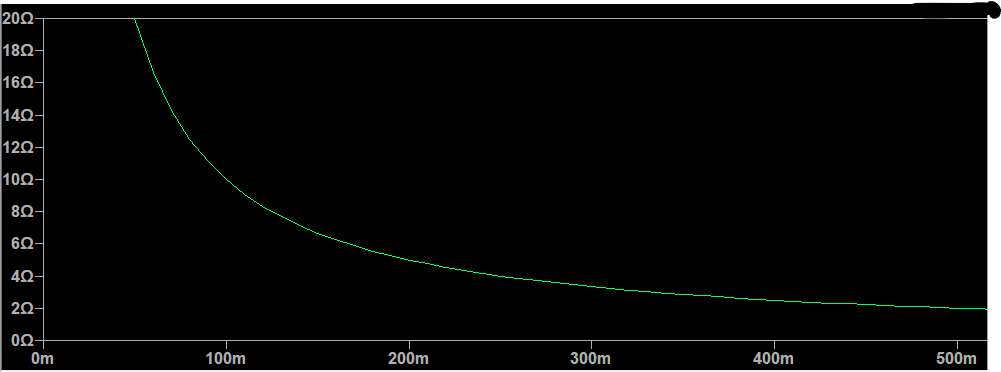
\includegraphics[width=0.2\textwidth]{images/graf.png}
    \caption{$V_S$ cuando $k = ALGO$}
\end{figure}


\newpage

\section{Respuesta al Escalón}

En esta sección se desea estudiar la respuesta al escalón de la carga activa para conseguir de 
manera práctica la función transferencia del circuito. La respuesta al escalón 
es la reacción de un sistema cuando recibe un cambio brusco de entrada, generalmente de cero a un valor 
constante. En este caso, se implementará un escalón de k para conseguir la función transferencia dada 
por la entrada k y la salida $Y_i$, es decir, $H(s) = \frac{Y_i}{k}$.

Para llevar a cabo este experimento, se debe tener en cuenta que la carga activa es un circuito 
que permite controlar una resistencia variable. Si se recuerda, dependiendo de dónde se coloque el 
cursor del potenciómetro, la resistencia de carga varía, y por lo tanto se puede hacer 
variar el divisor resistivo entre la fuente y el terminal no inversor del opamp. 

Como se mencionó anteriormente, se denominará k no solo a la posición del cursor, sino también al 
factor que multiplica al divisor resistivo. Por lo tanto, se puede pensar a k como una constante. 
Esta constante, si no se encuentra alterada por una resistencia en paralelo, es solamente la posición
del cursor. Sin embargo, si se coloca una resistencia en paralelo al potenciómetro, esta constante 
cambiará, incluso si se mantiene en el mismo lugar la posición del cursor.

De esta manera es como se implementará el escalón de k. Se colocará una resistencia en paralelo al 
potenciómetro, y se colocará un jumper para poder activar o desactivar esta resistencia de manera 
inmediata. Así, se podrá estudiar la respuesta al escalón de la carga activa y se podrá obtener la
respuesta en frecuencia del circuito. Dependiendo de cómo es el gráfico resultante puede ser posible
que pertenezca a un sistema de primer orden o de segundo orden. Como se están tomando en consideración 
un amplificador operacional y un transistor, se espera que la respuesta sea de segundo orden.

Dependiendo del gráfico que resulte, se podrá aproximar la función transferencia del circuito. 
Existen distintos tipos de filtros conocidos que se pueden obtener dependiendo de la respuesta al 
escalón. Analizando el gráfico en el osciloscopio, y viendo las oscilaciones que se producen, se 
podrá determinar qué tipo de filtro es. 

Nos interesa conocer el comportamiento de esta configuración, explorando distintos parámetros importantes 
que se pueden estudiar mediante la respuesta de este circuito ante la entrada de un escalón. Recordar 
que cuando se dispone de componentes no lineales, la entrada de un escalón producirá un transitorio 
oscilatorio antes de que se que el sistema se estabilice.

Se presentan a continuación los parámetros que se buscan conseguir:

\begin{itemize}
    \item \textbf{Parámetros de la respuesta al escalón:}
        \begin{itemize}
            \item \textbf{Frecuencia de oscilación del transitorio}: Puede ser diferente para cada tipo 
            de filtro. En un sistema subamortiguado: $f_n = \alpha + jf_d$, lo que implica que:

            \begin{equation}
                f_d = f_n \cdot \sqrt{1 - \xi^2}
            \end{equation}
            \newpage

            \item \textbf{Tiempo hasta la amplitud pico}: Es el tiempo que tarda el transitorio en 
            llegar hasta la amplitud máxima de las oscilaciones. Se puede calcular mediante la siguiente
            fórmula:

            \begin{equation}
                t_p = \frac{1}{2f_d} = \frac{1}{2 f_n \sqrt{1 - \xi^2}}
            \end{equation}

            \item \textbf{Sobrepico ($M_{pt}$)}: Este parámetro puede ser significativo para los filtros 
            pasabajos y pasaaltos con respuesta subamortiguada. Su magnitud depende del coeficiente de 
            amortiguación $\xi$.

            \begin{equation}
                M_{pt} = exp(\frac{-\pi \xi}{\sqrt{1-\xi^2}})
            \end{equation}

        \end{itemize}
\end{itemize}

Una vez obtenidos estos parámetros, se podrá determinar aproximar el tipo de filtro que se está utilizando, 
y además se podrá derivar la función transferencia que estamos buscando. Con la información obtenida 
mediante la respuesta al escalón, se podrán determinar los valores de $\xi$ y $f_n$, y se podrá 
aproximar la función transferencia del circuito.

Un ejemplo de una función transferencia de segundo orden es el filtro pasabajos. Este filtro se 
caracteriza por tener la siguiente función transferencia:

\begin{equation}
    H(s) = G_0 \cdot \frac{1}{(\frac{s}{\omega_n})^2 + 2\xi \cdot \frac{s}{\omega_n} + 1}
\end{equation}

Donde $G_0$ es la ganancia constante del filtro, $\omega_n$ es la frecuencia natural, y $\xi$ es el 
factor de amortiguamiento. Notar que: $\omega_n = 2\pi \cdot f_n$ y $Q = \frac{1}{2Q}$.

En este experimento, se espera ver un factor de amortiguamiento menor a 1, por lo que se verá un 
sistema subamortiguado. Por lo tanto, se espera que la respuesta al escalón sea oscilatoria, y que
se pueda aproximar la función transferencia del circuito midiendo los parámetros mencionados anteriormente.













\newpage

\section{Impedancia de Salida}
\subsection{Análisis Teórico y Predicciones}
Dentro de las distintas utilidades que puede tener un circuito como el estudiado en este trabajo práctico,
se encuentra la de poder calcular la impedancia de salida de una fuente de alimentación, o un generador de 
señales. En definitiva, es posible calcular la impedancia de salida de cualquier circuito que pueda mostrarse 
como un circuito equivalente de Thévenin o Norton por donde pase una corriente máxima de 3A. 

La impedancia de salida es una característica clave para evaluar cómo un circuito entrega su señal a un componente 
siguiente. Una impedancia de salida alta puede indicar que el circuito tiene dificultades para 
suministrar toda su tensión nominal, teniendo una significante caída en la resistencia interna, 
mientras que una impedancia de salida baja significa que el circuito puede proporcionar más corriente 
sin mucha pérdida de voltaje.

Matemáticamente, la impedancia de salida se define como:

\begin{equation}
    Z_{out} = \frac{V_{out}}{I_{out}}
\end{equation}

Donde $V_{out}$ es la tensión de salida y $I_{out}$ es la corriente de salida que circula. Para poder calcular
la impedancia de salida de una fuente, es necesario pensar a la misma como un circuito equivalente de
Thévenin. Este circuito consta de una fuente de tensión $V_{TH}$ en serie con una impedancia $Z_{TH}$.
Se puede pensar también a la fuente como un circuito equivalente de Norton, que consta de una fuente de
corriente $I_{N}$ en paralelo con una resistencia $R_{N}$. 

De esta manera, se pueden calcular las impedancias 
de salida de ambas fuentes. Para una mejor comprensión, se llevará a cabo esta explicación teniendo en 
cuenta que lo que se mide es una fuente de Thévenin. Se llamará a la señal generada por la fuente 
$V_{TH}$, mientras que su resistenica interna, o impedancia de salida, será $Z_{TH}$.

A continuación se presenta el circuito que se utilizará para calcular la impedancia de salida de la fuente:

\begin{figure}[H]
    \centering
    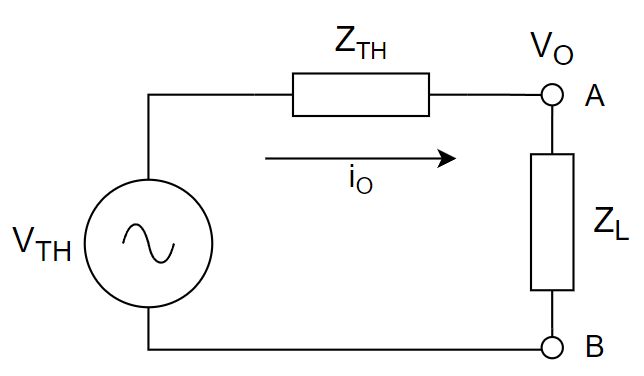
\includegraphics[width=0.6\textwidth]{images/thevenin.png}
    \caption{Equivalente de Thevenin}
\end{figure}

\newpage
Para llevar a cabo este experimento, se debe colocar entre los bornes A y B el circuito estudiado en 
el trabajo práctico: la carga activa. La impedancia $Z_L$ será una impedancia variable que podrá ser 
modificada mediante el cursor del potenciómetro. Para medir con precisión la impedancia de salida una 
fuente, es necesario imponer una señal de prueba en dicha fuente. Por ejemplo, para este experimento, 
se decidió utilizar una fuente de tensión continua y se impondrá una señal de prueba de 10V.

Se debe tener en cuenta que la resistencia interna de una fuente de tensión debe ser pequeña para que
la fuente pueda suministrar la mayor parte de su tensión nominal. El objetivo de la fuente de tensión 
es entregar toda esa tensión, y lo que hace la resistencia interna, dependiendo de la corriente que 
circule, es causar una caída de tensión en la misma. Como pudimos ver en este trabajo práctico, 
la carga activa permite controlar una impedancia dependiendo de la posición del cursor.
Esta impedancia devuelve para la mayoría de los casos una resistencia cercana a 1$\Omega$. Si se 
mantiene el cursor entre 0,1 y 1, la impedancia de carga tendrá valores entre 1 y 10$\Omega$.

Es importante aclarar que la tensión de prueba aplicada tendrá una magnitud de 10V pico. Dado que se 
espera que la resistencia interna de la fuente no supere los 10$\Omega$, la corriente que 
circula por el circuito podrá superar tranquilamente 1A. Por lo tanto, se debe tener en cuenta
que para llevar a cabo este experimento es fundamental el circuito propuesto con el mosfet y opamp 
ya que se consigue una resistencia variable que resiste corrientes en el orden de los amperes.
Por lo tanto, esta resistencia permitirá detectar impedancias de salida muy chicas como también grandes.

Si se observa en la figura anterior, se forma un divisor resistivo entre la resistencia de carga y la 
impedancia de salida de la fuente. Por lo tanto, se puede llegar a la siguiente ecuación:

\begin{equation}
    V_o = V_{th} \cdot \frac{Z_{L}}{Z_{TH} + Z_L}
\end{equation}

De esta manera, se puede inferir que si la tensión de salida es igual a la mitad de la tensión de la fuente,
entonces las impedancias son equivalentes. Puede verse esto mismo a través de las siguientes igualdades:

\begin{equation}
    V_o = \frac{V_{th}}{2} \implies \frac{V_{th}}{2} = V_{th} \cdot \frac{Z_{L}}{Z_{TH} + Z_L} 
    \iff 2Z_{L} = Z_{TH} + Z_L \iff Z_{TH} = Z_L
\end{equation}

Por lo tanto, se concluye que si la tensión de salida es la mitad de la tensión de la fuente, entonces
la impedancia de salida de la fuente es igual a la impedancia de carga. De esta manera, se puede calcular 
dicha impedancia de manera experimental mediante la ayuda de un osciloscopio o distintos 
instrumentos de medición haciendo variar la resistencia de carga mediante el cursor del potenciómetro.

Si bien este experimento permite encontrar impedancias de salida de algunas fuentes, es importante 
tener en cuenta que no es un método exacto. Esto se debe a que hay que tener mucha precisión en la 
rotación del cursor. Por ejemplo, si la resistencia interna de una fuente fuera de 50$\Omega$, se 
debería colocar el cursor en $k = \frac{1}{50}$ lo cual no es una tarea fácil ni exacta. Luego 
de conseguir el valor más cercano donde la tensión de salida es la mitad de la tensión de la fuente, 
se debe medir la resistencia de carga empleando el mismo experimento que se
llevó a cabo para encontrar la impedancia de entrada.

\subsection{Mediciones experimentales}

Para llevar a cabo este experimento, se utilizó una fuente de continua que se encuentra en el 
laboratorio de electrónica, y la carga activa propuesta en este trabajo práctico, sin la resistencia
de compensación o la necesitada para construir el escalón de k. Se utilizó un osciloscopio para 
medir la tensión de salida, y se varió la resistencia de carga mediante el cursor del potenciómetro.

Estableciendo una tensión de prueba de 10V, se midió la tensión de salida para distintas posiciones 
del cursor, pero no se pudo llegar a un valor donde la tensión de salida sea la mitad de la tensión 
de la fuente. En cambio, se encontró que la tensión mínima de salida era de .......

Por lo tanto, se puede concluir que la fuente de tensión utilizada en este experimento tiene una 
impedancia de salida menor a 1$\Omega$. Usualmente, se esperan que las fuentes de tensión tengan 
una resistencia interna menor a 1$\Omega$ para que puedan suministrar la mayor parte de su tensión 
a una carga, por lo que es un resultado esperado y coherente que no se haya conseguido 
una tensión de salida igual a la mitad de la tensión de la fuente.

\subsection{Alternativas de Medición}

Ya que no se pudo encontrar la impedancia de salida de la fuente de alimentación por el hecho de 
que la impedancia de carga era muy grande en comparación a la misma, se proponen alternativas que 
permiten mejorar esta medición. Si se desea medir la impedancia de salida de una fuente de tensión 
de manera más precisa, se pueden implementar distintos métodos.

\subsection*{Método 1}

Una de las alternativas se basa en fijar el cursor k en un valor específico, y medir la tensión de 
salida que presenta el circuito ante esta configuración. Se puede elegir, por ejemplo, un valor de 
k = 1, ya que es fácil de establecer este valor. De esta manera, se tienen como datos la resistencia 
de carga y la tensión de salida. 

Luego, se debe encontrar la tensión que proporciona directamente la fuente, sin la intervención 
de la resistencia interna. Pero, ¿es esto posible? La resistencia interna de la fuente está 
físicamente dentro de la fuente, por lo que no es posible medirla directamente. Sin embargo, 
sí se puede llevar a cabo un experimento que dicte aproximadamente cuál es la tensión nominal 
que proporciona la fuente. Si se coloca un voltímetro en paralelo con la fuente, se está cerrando 
el circuito con este instrumento de medición. 

El voltímetro tiene una resistencia interna 
considerablemente grande, idealmente infinita, para que no circule corriente por esa rama. 
Por lo tanto se está cerrando el circuito con una corriente muy baja, por lo que la tensión 
que se está midiendo es la tensión de la fuente sin la intervención de la resistencia interna.
A continuación se presenta el circuito en cuestión:

\begin{figure}[H]
    \centering
    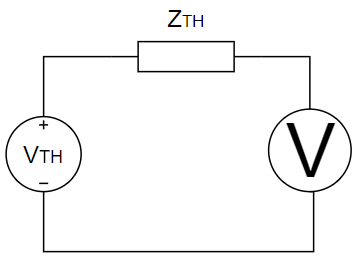
\includegraphics[width=0.45\textwidth]{images/voltimetro.png}
    \caption{Método 1}
\end{figure}

De esta manera, se obtiene la tensión que proporciona la fuente. Como se mencionó anteriormente, 
la tensión de salida es un divisor resistivo entre la resistencia de carga y la impedancia de salida
dado por:

\begin{equation}
    V_o = V_{TH} \cdot \frac{Z_{L}}{Z_{TH} + Z_L}
\end{equation}

Teniendo sólo como incógnita la impedancia de salida, se puede despejar la misma para encontrar su 
valor:

\begin{equation}
    Z_{TH} = \frac{V_{TH}Z_L}{V_o} - Z_L
\end{equation}

De esta manera, se puede encontrar la impedancia de salida de la fuente de tensión de manera aproximada. 
Sin embargo, es importante destacar que este experimento solo puede llevarse a cabo con un valor de 
k = 1, ya que no se puede encontrar de otra manera el valor de k exacto que se está utilizando.
Si k = 1 sabemos el valor de la impedancia de entrada de la carga activa, pero está circulando la 
corriente máxima que puede soportar el circuito. 

Es preferible implementar mediciones donde no se esté dependiendo de parámetros no certeros como 
puede ser la posición del cursor, o también el funcionamiento del MOSFET y el opamp. Por lo tanto, 
se propone un segundo método para poder medir la impedancia de salida de la fuente de tensión 
de manera más precisa y certera, sin depender de la posición del cursor.

\subsection*{Método 2}

El segundo método propuesto se basa en la utilización de varios instrumentos de medición para poder 
calcular la corriente que circula por el circuito cuando la carga activa está conectada, y con un 
valor de k cualquiera. Se propone hacer las mediciones con dos voltímetros: uno para medir la caída de 
tensión en la resistencia de 1$\Omega$, y otro para medir la tensión de salida, es decir, la tensión que 
entra a la carga activa.

A continuación puede verse el circuito propuesto para llevar a cabo este experimento:

\begin{figure}[H]
    \centering
    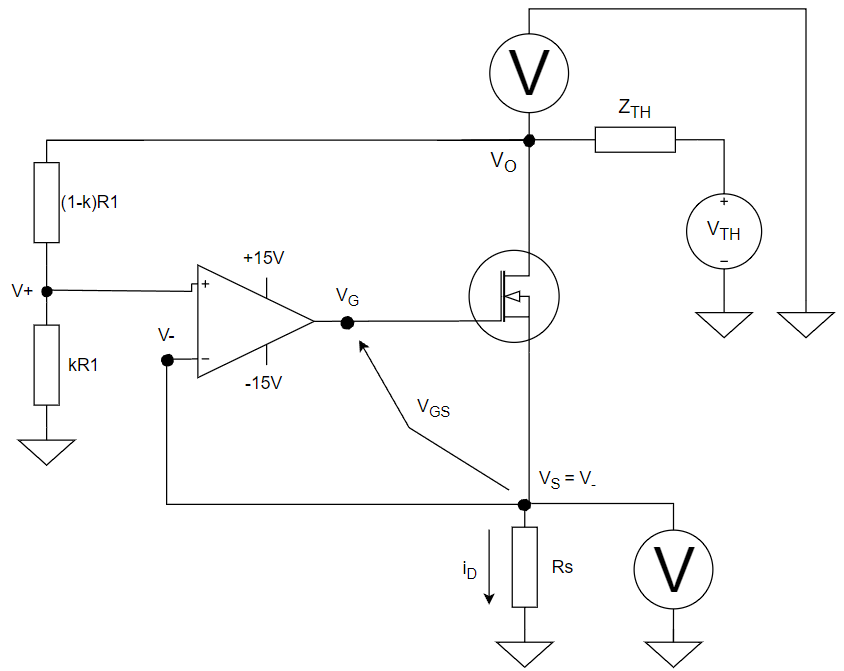
\includegraphics[width=0.8\textwidth]{images/voltimetros.png}
    \caption{Método 2}
\end{figure}

Para simplificar y comprender mejor el circuito, se puede pensar el circuito como la \enquote*{Figura COMPLETAR LO QUE QUEDE},
es decir, como un equivalente de Thévenin conectado a una resistencia de carga. Los voltímetros serán 
utilizados en este experimento para medir: $V_S$ y $V_o$. 

Con $V_S$, se puede saber el valor de la corriente que circula por el circuito, es decir, $I_D$. 
Se obtiene mediante la siguiente fórmula: $I_D = \frac{V_S}{R_S}$, donde $R_S$ es la resistencia de 
1$\Omega$. Por otro lado, con $V_o$ se puede saber la tensión de salida que proporciona la fuente 
luego de pasar por la impedancia de salida.

De esta manera, se puede calcular la impedancia de salida de la fuente de tensión mediante el 
siguiente divisor resistivo:

\begin{equation}
    V_o = V_{TH} \cdot \frac{Z_{L}}{Z_{TH} + Z_L}
\end{equation}

Donde $Z_L$ es la resistencia de carga que ve el equivalente de Thévenin. Es decir, que: 

\begin{equation}
    Z_L = \frac{V_o}{I_D} = \frac{V_o}{\frac{V_S}{R_S}} = \frac{V_o \cdot R_S}{V_S} = \frac{V_o}{V_{S}}
\end{equation}

Si bien se logró encontrar una expresión para calcular la impedancia de salida de esta fuente sin 
depender de k, es importante destacar que este método no permite hacer el cálculo mediante sólo una 
medición. Como se puede ver en la \enquote*{Ecuación 38}, tenemos dos incógnitas: $V_{TH}$ y $Z_{TH}$.

Por lo tanto, se necesitarán dos mediciones como mínimo para poder implementar este método correctamente.
Se propone establecer el cursor del potenciómetro en dos posiciones al azar y medir las tensiones 
correspondientes. Como consecuencia, se pueden observar las siguientes expresiones:

\begin{equation}
    V_{o_1} = V_{TH} \cdot \frac{Z_{L_1}}{Z_{TH} + Z_{L_1}}
\end{equation}

\begin{equation}
    V_{o_2} = V_{TH} \cdot \frac{Z_{L_2}}{Z_{TH} + Z_{L_2}}
\end{equation}

Luego, dividiendo ambas ecuaciones, se obtiene: 

\begin{equation}
    \frac{V_{o_1}}{V_{o_2}} = \frac{Z_{L_1}\cdot (Z_{TH} + Z_{L_2})}{Z_{L_2}\cdot (Z_{TH} + Z_{L_1})}
\end{equation}

Despejando $Z_{TH}$ se obtiene:

\begin{equation}
    Z_{TH} = \frac{Z_{L_1} - C\cdot Z_{L_2}}{C - 1} \iff C = \frac{V_{o_2} Z_{L_1}}{V_{o_1} Z_{L_2}}
\end{equation}

Notar que C es una constante que no puede ser igual a 1, ya que es una discontinuidad de la 
ecuación \enquote*{Ecuación 43}.

Como se puede ver en la serie de ecuaciones presentadas, se puede calcular la impedancia de salida 
de la fuente de tensión sin tener en cuenta el parámetro k. Sin embargo, es importante destacar que 
es necesario que las mediciones sean distintas, es decir, que no se use el mismo valor de k para 
realizar el experimento.

\subsection{Cálculo de la Impedancia de Salida}

Para llevar a cabo este experimento, se propone utilizar el método 2, ya que es más preciso y 
no depende de la posición del cursor. Se realizarán mediciones con el osciloscopio para poder
calcular la impedancia en cuestión. Se posicionará el cursor en dos valores distintos de k, cercanos 
al 0,5 pero no iguales. Se medirán las tensiones $V_{S_1}$, $V_{S_2}$, $V_{o_1}$ y $V_{o_2}$.

A continuación se presenta una tabla con los valores obtenidos en el laboratorio:

\begin{table}[H]
    \centering
    \begin{tabular}{|c|c|c|c|}
        \hline
        \rowcolor[HTML]{C0C0C0} 
        \hline
        \textbf{$V_{S_1}$ (V)} & \textbf{$V_{S_2}$ (V)} & \textbf{$V_{o_1}$ (V)} & \textbf{$V_{o_2}$ (V)} \\ \hline
        0,5                   & 0,5           & 0,5           & 0,5           \\ \hline
        0,5                   & 0,5           & 0,5           & 0,5           \\ \hline
    \end{tabular}
    \caption{Tensiones medidas}
\end{table}

Una vez obtenidos estos valores, se pueden calcular las impedancias de carga debida la carga activa de 
cada caso. Luego, se puede calcular la impedancia de salida de la fuente de tensión mediante la 
\enquote*{Ecuación 43}.

En la siguiente tabla se presentan los valores restantes, como también la impedancia de salida resultante:

\begin{table}[H]
    \centering
    \begin{tabular}{|c|c|}
        \hline
        \rowcolor[HTML]{C0C0C0} 
        \hline
        \textbf{Impedancia} & \textbf{Valor ($\Omega$)} \\ \hline
        \textbf{$Z_{L_1}$}         & 0,5             \\ \hline
        \textbf{$Z_{L_2}$}         & 0,5             \\ \hline
        \textbf{$Z_{TH}$}          & 0,5             \\ \hline
    \end{tabular}
    \caption{Impedancias calculadas}
\end{table}

\subsection*{Conclusión}

Como se puede observar en la tabla anterior, se obtuvieron valores experimentales de una impedancia de 
salida de la fuente utilizada, que antes era imposible de medir directamente. Una vez obtenida la 
impedancia de salida de la fuente, se pueden predecir comportamientos a futuro con esta misma fuente, ya 
que si se coloca una resistencia de carga de, por ejemplo, 500m$\Omega$, esta no será despreciable 
en comparación a la de la fuente, por lo que habrá una caída de tensión considerable en la misma.

Es esencial la utilidad de la carga activa para medir impedancias de salida, ya que permite 
averiguar cómo se comportan algunas fuentes cuando se les conecta una carga. Sea la impedancia 
de salida que sea, esta puede ser calculada mediante este experimento. Ya fuera de manera 
aproximada o precisa, se puede obtener un valor para la misma. 

Si se quisiera encontrar una medida más exacta de la impedancia de salida de una fuente, podría 
repetirse este proceso infinitas veces con distintos valores de k, y se podría hacer un promedio 
de todas las impedancias obtenidas. De esta manera, se podría obtener un valor más certero de la 
impedancia de salida de la fuente de tensión.


\newpage

\section{Bibliografía}

\nocite{*}
    \printbibliography


\end{document}